\makeatletter
\def\@makeschapterhead#1{%
  \vspace*{10\p@}%
  {\parindent \z@ \centering \normalfont
      {\includegraphics[scale=1]{om.eps}}\\[10pt]
      {\Large\bf shirxV shirxVraMgasadugxraveV namaH}\\[10pt]
      %\par\nobreak
      %\vskip 5\p@    
    \interlinepenalty\@M
    \huge \bfseries  #1\par\nobreak
    \chaptermark{#1}
    \vskip 20\p@
  }}
\makeatother

\chapter*{parxkAshakara nuDi}

{\addTOCLine{parxkAshakara nuDi}}

shirxVraMga mahAgurugaLa parxvacanagaLa saMkalanavAda amaravANiV 11 neya \hbox{saMpuTa} ``saMsakxqqta-saMsakxqqti" eMba garxMthada karaDuparxtiyanunx utAthxna dAvxdashiyaMdu shirxVmAteyavarige samapaRNe mADi, avara AshiVvARda paDedu iMdu mudirxtarUpadalilx janateya muMdiDalu saMtoVSisutetxVve.

shirxV guruBagavaMtaru kuLitAga, niMtAga, reYlinalilx parxyANa mADutitxdAdxga, BoVjanada samayadalilx parxshenxgaLaninxTATxga, nAvugaLu sikikxdAga namamxgaLa shikaSxNakAkxgi saMsakxqqtige saMbaMdhisida mAtugaLanunx ADutatxleV idadxru. navarAtirxkAladalilx, beVsige rajadalilx elalxrU oTiTxge seVridAga (samemxVLanagaLalilx) basariVkaTeTxya sadugxru vidAyxshAleyalilx pATharUpavAgi parxvacanagaLanUnx anugarxhisidUdx uMTu. 

aneVka pATha parxvacanagaLanunx keVLidadxrU, avara vicAradhAreyanunx garxhisalu kaSaTxvAgutitxdudxdariMda, oMdu cwkaTiTxnalilx pAThagaLanunx namage iTaTxre, namage garxhisalu sulaBavAgutatxdeMba pArxthaRneyanunx nAnomemx iTATxga tatAkxladalelxV mUlaBUtavAda viSayagaLa bagegx hinenxle pAThavanAnxraMBisidaru. sUkxlu, kAleVju, APiVsugagaLalilx hAgU saMsakxqqtapAThashAleyalilx kelasamADutitxdadx namamxgaLa virAma kAlagaLalilx aMdare shanivAra, BAnuvAra, hAgU sAvaRtirxka rajAdinagaLu- pAThashAlege anadhayxyana rajAdinagaLu oTiTxge seVri baMdAga, pAThagaLanunx muMduvarisuva yoVjane sidadhxvAyitu.  kelavu hiriya sadasayxranunx Ayekx mADikoMDu avarugaLige pAThavaninxTuTx avariMda itara sadasayxrige pAThaviDisabeVkeMbudU I yoVjaneya aMgavAyitu. idaraMte naDeda kelavu mUlaBUta pAThagaLanunx `` ASaRvideyxgaLa mwlikate" eMba shiVSiRkeyalilx I saMpuTadalilx koDalAgide. I pAThagaLigeV seVrida `dashaRna' (``jiVvanadalilxya noVTa") eMba pAThavu amaravANiV 1neya saMpuTadalilx `jiVvana dashaRna' eMba shiVSiRkeyalilx acAcxgiruvudariMda matetx I saMpuTadalilx adanunx seVrisilalx.

saMsakxqqta AyoVgada parxshAnxvaLige kaLuhisida utatxra hAgU shirxVmanamxhArAja jayacAmarAjeVMdarx oDeyaravaru keVLidadx parxshenxgaLige koTaTx utatxragaLu, saMsakxqqtige saMbaMdhisida aneVka mwlika saMgatigaLanunx oLagoMDiruvudariMda, avugaLanUnx I saMpuTadalilx seVrisalAgide.

namamx saMsethxge modalige `vijAcnxna maMdira' eMdu hesaranunx shirxVguruBagavaMtaru koTiTxdadxru. `vijAcnxna'da hiMde `aSATxMgayoVga' (jAcnxna) ideyeMbudanunx tiLisutitxdadxru. I parxvacanagaLalilx maMdiravanunx `vijAcnxnamaMdira' eMdeV ulelxVKiside. maMdiravanunx 1968 ralilx rijisaTxrf mADisuvAga ``aSATxMgayoVga vijAcnxna maMdiramf" eMba pUNaRvAda hesaranunx baLasalu shirxV gurudeVvaru anumati koTaTxru.

noVTusx hAgU mUlabarahagaLanunx parishiVlisi, I saMpuTadalilxna leVKanagaLanunx acicxgAgi sidadxpaDisi, aneVka saMsakxqqta mUlagaLige kananxDa BAvAnuvAdavanunx niVDi hAgU I saMpuTakekx BUmikeyanUnx saha barediruva namamx hiriya soVdara vidAvxnf enf. esf. rAmaBadArxcAyaRrige namamx kaqtajacnxtegaLu. I saMpuTada parxkAshanadalilx neravu niVDiruva vidAvxnf enf. esf. janAdaRnAcArayxru, iMDekfsx sidadhxpaDisuvudu, sholxVkagaLige BAvAnuvAda itAyxdiyAgi parxkAshanadalilx udadxkUkx neravu niVDiruva DA|| ke. elf. shaMkaranArAyaNa joVyisaru, citarxvoMdanunx baredukoTuTx seVve salilxsiruva ci|| haSaR siMha, savxlapxmaTiTxge AthiRka neravu niVDi, garxMthada beleyanunx kaDimeyAgiyeV iDalu sAdhayxvAguvaMte mADiruva soVdara ji. ke. shirxVnivAsamUtiR hAgU otAtxse niVDutitxruva maMdirada soVdara-soVdari vagaR-ivarelalxrigU kaqtajacnxtegaLu.

aMdavAgi mudarxNa mADi, sahakAra niVDiruva caMcu perxsisxna shirxV Arf. narasiMha avaru namamx kaqtajacnxtege pAtarxru.

elalxdakUkx migilAgi, namage sUPxtiR cilumeyAgi namamxnunx anugarxhisi huriduMbisutitxruva paramapUjayx vijayalakiSxmXV shirxVmAteyavarige pArxNa parxNAmagaLu.

\vskip 1cm

\noindent Ishavxra saMvatasxra \hfill shaMkaranArAyaNadAsa

\noindent veYshAKa shukalx EkAdashiV \hfill (shirxVkaMTha)

\noindent {(\rm 18--5--1997)} \hfill kAyaRdashiVR

